\documentclass{article}
\usepackage{amsmath}
\usepackage{amssymb}
\usepackage{hyperref}
\usepackage{fancyhdr}
\usepackage{graphicx}
\usepackage{setspace}
\usepackage{caption}
\usepackage{wrapfig}
\usepackage{cancel}
\usepackage{pythonhighlight}
\usepackage{float}
\usepackage[a4paper, total={6in, 8in}]{geometry} 
\usepackage{mdframed}
\usepackage{modalops}
\usepackage{mathrsfs}
\usepackage{tikz}


\graphicspath{C:\Users\cmark\OneDrive\Documents\Latex}


\hypersetup{
    colorlinks=true,
    linkcolor=blue,
    urlcolor=cyan,
    citecolor = red
}

\pagestyle{fancy}
\renewcommand{\headrulewidth}{0.4pt}
\renewcommand{\footrulewidth}{0.4pt}
\setlength{\headheight}{18pt}
\setlength{\parindent}{12pt}

\lhead{\large{\bf Carter Garrett}} 
\chead{}
\rhead{\textsc{PHIL 305, Philosophy of Logic 5}} 
\lfoot{\today}
\cfoot{}
\rfoot{} 

\newmdtheoremenv{task}{Task}

\usetikzlibrary{arrows,calc,patterns,positioning,shapes}
\usetikzlibrary{decorations.pathmorphing}
\tikzset{
modal/.style={>=stealth',shorten >=1pt,shorten <=1pt,auto,
node distance=1.5cm,semithick},
world/.style={circle,draw,minimum size=1cm,fill=gray!15},
point/.style={circle,draw,fill=black,inner sep=0.5mm},
reflexive/.style={->,in=120,out=60,loop,looseness=#1},
reflexive/.default={5},
reflexive point/.style={->,in=135,out=45,loop,looseness=#1},
reflexive point/.default={25},
}


\newcommand*\fancypants{\vcenter{\hbox{\includegraphics[width = 2.0em]{fp.png}}}}

\begin{document}

    \section{First Formula}
    \begin{task}
        Discuss whether we should accept the following: 
        \begin{center}
            If $\Gamma \vDash C$ then $A \necif B$ : $B \in \Gamma \vDash A \necif C$   
        \end{center}
    \end{task}

    The statement can be read as:
    If $C$ can be obtained from $\Gamma$, then $A \necif B$. 
    And if $B$ is an element of $\Gamma$, then $A \necif C$.
    A closer inspection might yield: 

    \begin{enumerate}
        \item $\Gamma \vDash C$ will produce $A \necif B$. Meaning, that $V_{\mathscr{M},g}(B, w) = 1$ at the maximally close $A$ world $w$, only if $\Gamma \vDash C$.
        \item Since $B$ is true at $w$, and since $B \in \Gamma$, we can get $C$ from $\Gamma$ since we have $B$.
        \item Therefore, $C$ must also be true at $w$, which is the maximally close $A$ world.
        \item $\therefore \; A \necif C$.
    \end{enumerate}

    

    \subsection{Motivations and Investigation}  

        Kai Von Fintel discusses an important aspect of counterfactuals that is relevant here. 
        In Section 6 \cite{fintel}, he discusses the excluded middle in the context of counterfactuals. 
        Typically, it would seem very natural to accept a statement like $(\phi \vee \lnot \phi)$, though even this is subject to scrutiny.
        Fintel points out that on Stalnaker's calculus for evaluating counterfactuals, the \textit{uniqueness assumption} creates a system in which the law of the excluded middle is valid.

        Specifically, on Stalnaker's view, the truth conditions for $(\phi \necif \psi)$ are such that only one $\phi$ world maximally similar to the actual world exists. 
        As an example model, we might have something like: 

        \begin{figure}[H]
            
            \begin{center}
                \begin{tikzpicture}[modal]
                    \node[world] (w) [label=below:$@w$] {};
                    \node[world] (v) [label=below:$v$,below right=of w, xshift= -5mm, yshift = 5mm] {$\phi, \psi$};
                    \node[world] (u) [label=below:$u$,below left=of w] {$\phi$};
                    \node[world] (s) [label=below:$s$,above right=of w] {$\phi$};
                    \node[world] (r) [label=below:$r$,above left = of w] {$\phi$};
                    
                    \path[<->] (r) edge (w);
                    \path[<->] (w) edge (s);
                    \path[<->] (w) edge (v);
                    \path[<->] (w) edge (u);
                    %\path[->] (w) edge[reflexive] (w);
                \end{tikzpicture}
            \end{center}
        \caption{A sample world model using Stalnaker's counterfactual system.}
        \end{figure}\label{fig1}
        
        In Figure \ref{fig1}, it is clear that $v$ is the maximally similar $\phi$ world. Since it is unique, it is only possible that $\psi$ or $\lnot \psi$ will obtain for that world $v$. 
        So the excluded middle holds in this case. It is clear that $V_{\mathscr{M}, g}(\phi \necif \psi, w) = 1$. 

        But the Lewis system for counterfactual evaluation, the truth conditions are such that $LV_{\mathscr{M}, g}(\phi \necif \psi, w) = 1$ 
        iff there is some world $u$ s.t. $LV_{\mathscr{M},g}(\phi, u) = 1$ and for every $\phi$ world $v \leq_w u$, $LV_{\mathscr{M}, g}(\psi , v) = 1$ \footnote{The truth conditions in the notes have typos, I believe this is what the condition meant to be.}.
        For Lewis, we may have lots of similar $\phi$ worlds equidistant from the actual world, for which $\psi$ may be true. But there may be other set members missing or present in those worlds, which affect the conclusion of the counterfactual.

        Let's frame the original statement in a model: 

        \begin{figure}[H]
            \begin{center}
                \begin{tikzpicture}[modal]
                    \node[world] (w) [label=below:$w$] {$\Gamma$};
                    \node[world] (u) [label=below:$u$, left = of w] {$A, B, C$};
                    \node[world] (s) [label=below:$s$, right = of w] {$A, B, Q$};

                    \path[<->] (w) edge (u);
                    \path[<->] (w) edge (s);
                \end{tikzpicture}
            \end{center}
            \caption{Two equally similar $A$ worlds, and deductions.}
        \end{figure}\label{fig2}

        In Figure \ref{fig2}, we see that $A \necif B$ obtains for two \textit{equally similar} worlds. But $C$ does not necessarily obtain for both of them, although $B$ is a member of set $\Gamma$.
        There may be a case where not \textit{all closest A worlds} validate $C$. On this view, it seems we should not accept the first formula.
        
        We can also consider this formula in the context of Fintel's section 3 \cite{fintel}. In that section on nonmonotonicity, he argues that strengthening the antecedent will not always evaluate to the same counterfactual conclusion.
        Moreover, he argues that hypothetical syllogisms (transitivity) fails for counterfactuals. In his example \cite{fintel}:

        \begin{enumerate}
            \item If Hoover had been born in Russia ($A$), he would have been a Communist ($B$).
            \item If Hoover had been a Communist ($B$), he would have been a traitor ($C$).
            \item $\nrightarrow$ If Hoover had been born in Russia, he would have been a traitor ($B \necif C$).
        \end{enumerate}

        This is reminiscent of our first formula-- $A \necif B$ where it is possible for $C$ to obtain from $\Gamma$, it doesn't guarantee that $A \necif C$ will be the case as well.
        There may be some instance where Hoover, having been born in Russia, falls in love with the American democracy and pledges his allegiance after immigrating $A \necif P$, and is not a traitor.
        So we cannot completely accept transitivity, though there may be some cases, where the uniqueness assumption is granted, that allow for us to accept it.
        But both Lewis and Stalnaker accept that in the case where there are no similar $A$ worlds, $B$ would obtain and therefore $C$ for the counterfactual.



    \section{Second Formula}
    \begin{task}
        Discuss whether we should accept the following:
        \begin{center}
            $\vDash (A \necif C) \vee (A \necif \lnot C)$
        \end{center}
    \end{task}

    \subsection{Motivation and Investigation}
    Again, Kai Von Fintel highlights some important elements between the Lewis and Stalnaker methods for evaluating counterfactual claims. In Sections 3 and 6 \cite{fintel}, it is important to acknowledge the fulness of the limit assumption.
    While the limit assumption prompts the uniqueness assumption, it also implies something like the following: 
    
    \begin{center}
        \textit{``Worlds can become asymptotically closer to the actual world-- there is a limit to the closeness of those worlds.''}
    \end{center}

    If there is an actual limit to similarity between worlds, then it would seem that for any counterfactual claim like $A \necif C$, there would be some limit towards $C$ or $\lnot C$. 
    Stalnaker accepts the limit assumption, and given that there is a unique, maximally similar world, the law of the excluded middle holds as well. 
    It would seem for Stalnaker, the second formula is valid.

    But Lewis asserts that we have no real obligation to accept the limit assumption.
    Take an example cited by Fintel \cite{fintel}:

    \begin{center}
        \textit{``If the one inch line had been slightly longer...''}
    \end{center}

    For any finite length of line we take that is longer than one inch, \textbf{there will always be a shorter line that is longer than one inch}.
    Sure, a mathematician might say that the limit of these lines approaches one inch-- but then we have no counterfactual claim.
    We need to consider lines that are longer than one inch, but so infinitessimally close. And for any one of those lines, we can say there is a more similar line. 
    This is problematic, because this would mean that there is not a maximally similar world, and we would not be compelled to accept $C$ or $\lnot C$ for $(A \necif C \vee A \necif \lnot C)$! 

    As a continuation on the uniqueness assumption, there are instances where we would want to accept the equal plausibility of two equally similar worlds. 
    
    \begin{enumerate}
        \item ``If Carter made new friends, he would have adopted his friends' hobbies.''
        \item ``If Carter made new friends, the friends would have adopted Carter's hobbies.''
    \end{enumerate}

    Each world seems equally plausible-- we would want to accept both. But the law of excluded middle would forbid it. 
    So it seems, along with Lewis's rejection of the uniqueness assumption, we should also reject formula 2 for counterfactuals.
    This example is similar to David Lewis's example of Bizet and Verdi \cite{lewis}.

    \begin{center}
        Thank you Joseph, Hannah, Atticus, and Dr. Haderlie for the awesome semester.

        $$\fancypants$$
    \end{center}
    \newpage
    \bibliographystyle{plain}
    \nocite{*}
    \bibliography{refs}

    
\end{document}